\documentclass[12pt,onecolumn]{article}
\usepackage{graphicx}
\usepackage{hyperref}
\usepackage{url}
\usepackage{wrapfig}
\usepackage{tikz}
\usepackage{caption}
\usepackage{subcaption}
\usetikzlibrary{shapes}
\usetikzlibrary{positioning}

\newcommand{\horrule}[1]{\rule{\linewidth}{#1}}

\title{\huge Tracking Interconnected Facebook Links - Project Report}

\author{ \horrule{1pt} \\ \textbf{ELEN4009 - Software Engineering} \\ \emph{School of Electrical and Information Engineering,} \\ \emph{University of the Witwatersrand,} \\ \emph{Johannesburg, South Africa} \\ \horrule{1pt} \\\\ \emph{Back-End Pair:} \\ Julian Zeegers (704582) \\ James Allingham (672732) \\ \\ \emph{Front-End Pair:} \\ Joseph Gage (751052)\\ Nathan Haag (873666) \\ \horrule{1pt}}

\addtolength{\oddsidemargin}{-0cm}
\addtolength{\evensidemargin}{-.0cm}
\addtolength{\textwidth}{0cm}


%%%%%%%%%%%%%%%%%%%%%%%%%%%%%%%%%%%%%%%%%%%%%%%%%%%%%%%%%%%%%%%%%%%%%%%%%%%%%%%
\begin{document}

\date{\vspace{-5ex}}
\maketitle
\pagestyle{plain}
\thispagestyle{empty}

\begin{abstract}
Your abstract goes here...
...
\end{abstract}

\newpage

\tableofcontents
\listoffigures
\listoftables
\thispagestyle{empty}
\setcounter{page}{0}

\newpage

\section{Introduction}

	\subsection{Problem Statement} % James

	Facebook is one of the most popular social networks used today. Due to the fact that it has over 1.5 billion users, it produces an incredibly large amount of data \cite{fb}. This data could be used in a number of ways:

	\begin{itemize}
		\item Data scientists and analysts could make use of this data to learn about social trends.

		\item Individuals can use the data for personal analytics.

		\item Sociologists to use the data to make and test new hypotheses.

		\item Marketing and advertising agencies could create specialized and targeted adds depending on a set of user's likes and status updates.

	\end{itemize}    

	There are a large number of potential applications and the possibilities are only constrained by human creativity.

	The Tracking Interconnected Facebook Links project is intended to visualize the links and connections of a Facebook user with other users. Initially, these visualisations are focused on identifying the relationships of a Facebook user (the end user of this product) with the network of friends this Facebook user has. The visuals are also intended to further illustrate the relationship connections of the user's friends of friends and an overview of the user's friend network. Some personal analytics such as analyses of the user's Facebook post contents will also be implemented. There is a myriad of additional features that could be added to this tool and therefore the solution must be dynamic and flexible. For example degrees of separation analyses or more personal analytics. This document describes the software requirements that will ensure that the end product is of the highest quality, produced most efficiently and is created as close to the requirements as possible. At a later point the project could be expanded to include the large scale data analytics used by data scientists, sociologists and marketers. 

	The project team consists of four Software Engineering students, divided into two groups: one for the front-end and one for the back-end. This document serves as a description of the project. The software requirement specification will be laid out. The design and implementation of the front and back ends will be discussed. Finally, the Scrum planning and retrospective will be presented.

	\subsection{Project Objectives} % James

	In order to both quantify the success of the project as well as properly create tasks with correct priorities, the objective of the project must be laid out. They are as follows:

	\begin{itemize}

		\item Create a prototype system for visualizing a persons Facebook connections, social trends and personal analytics.

		\item Document the requirements for the system.

		\item Document the design of the system.

		\item Document the implementation and testing of the system.

		\item Document the group work aspects of the system including the SDLC.

	\end{itemize}

	\subsection{Stakeholders} % James

		The Project Management Body of Knowledge describes stakeholders as individuals or organizations that may be impacted in any way by the decisions or outcomes of a project \cite{pmbok}. There are a number of stakeholders whose interests must be considered when carrying out the objectives above. Often the stakeholders can have conflicting interests which must be compared and carefully weighed up in order to resolve the conflict. The following stakeholders are considered to be of paramount importance:

		\begin{itemize}
			\item \textbf{The Users}. The users of the system will be individuals who wish to explore their own personal Facebook friend networks and perform intimate personal analytics on their data. At this point the users \textbf{do not} include data scientists, analysts, sociologists and marketing/ advertising professionals - a later version of the software will be targeted at these groups. The reason that the individual was chosen as the first target market is that the requirements for the individual are much less resource intensive and thus are a more realistic goal for the first version of a product. Every decision that is made should improve the user's experience when interacting with the product. 

			\item \textbf{The development team}. The development team consists of four software engineering students. These four developers are then divided into two teams, the front-end team and the back-end team. It is important that the work in the project is divided appropriately between the teams. It is important to note that the Scrum SDLC does not make distinctions between different developers and so it is up to the developers themselves to choose the appropriate tasks that best fit their skill sets. The success or the failure of the project will have a large impact on the development team. On the other hand, the development team will have a large impact on whether or not the project is a success. Whenever a decision is made, it should be one that makes both the best use of the team as well as improves the likelihood that the project will be a success.

			\item \textbf{Facebook}. Although Facebook will not themselves be involved in the project, the perception of the company could be influenced by the product if it is successful. This could be as a result of people learning more about amount or type of data about them on Facebook.

		\end{itemize}

	\subsection{Abbreviations, Acronyms and Definitions} % All of us

	\begin{enumerate}
		\item \textbf{ACID} - Atomicity Consistency Isolation Durability. A model for reliable database systems.

		\item \textbf{Apache}. A popular web server.

		\item \textbf{Client-Server}. An architecture or model for distributed computing via the Internet or other network.

		\item \textbf{CSS} - Cascading Style Sheets. A style sheet language for describing the presentation of a website.

		\item \textbf{Cypher}. The query language for Neo4j graph databases.

		\item \textbf{d3.js}. A popular JavaScript library for visualisation.

		\item \textbf{DBMS} - Database Management System. A database program.

		\item \textbf{Django}. An MTV web application framework, written in Python.

		\item \textbf{Git}. A program for software and document version control.

		\item \textbf{GitHub}. A website for hosting git repositories.

		\item \textbf{GUI} - Graphical User Interface. A visual tool that allows a user to interact with an application.

		\item \textbf{HTML} - Hyper Text Markup Language. A markup language for creating web pages.

		\item \textbf{HTTP} - Hyper Text Transfer Protocol. An Application level protocol that makes use of HTML from sending and receiving messages in a client-server architecture.

		\item \textbf{JS} - JavaScript. A scripting language often used in building interactive applications in the Web 2.0.

		\item \textbf{JSON} - JavaScript Object Notation. A data interchange notation used extensively in web applications.

		\item \textbf{mod\_wsgi}. The Django module for Apache Web Server.

		\item \textbf{MTV} - Model Template View. Another name for the popular MVC framework. This is the nomenclature used by the Django web framework.

		\item \textbf{MVC} - Model View Controller. A framework for building web applications based on a three layer abstraction of the data, the presentation and the interaction between them. 

		\item \textbf{Neo4j}. A graph database written in Java.

		\item \textbf{Py2Neo}. A Neo4j driver for the Python programming language.

		\item \textbf{Python}. A popular, powerful and flexible scripting language.

		\item \textbf{Slack}. An application for team communication.

		\item \textbf{SDLC} - Software Development Life Cycle. The process or approach the software development team adheres to.

		\item \textbf{Trello}. A web application for managing project tasks.

		\item \textbf{UI} - User Interface. A tool allowing a user to interact with an application.

		\item \textbf{Web 2.0}. The informal name for websites that emphasize user generated content such as Facebook.


	\end{enumerate}

\section{Software Requirement Specification} % James

	\subsection{Introduction}
	This project is intended to visualize the links and connections of a Facebook user with other users. Initially, these visualisations are focused on identifying the relationships of a Facebook user (and the end user of this product) with the network of friends this Facebook user has. The visuals are also intended to further illustrate the relationship connections of the user's friends of friends and an overview of the user's friend network. There will be more features that could potentially be added to this tool and therefore the solution must be dynamic and flexible. This section describes the software requirements that will ensure that the end product is of the highest quality, produced most efficiently and fulfils its requirements.

	\subsubsection{Requirements}

	The requirements for the application are that it:
	\begin{enumerate}
	\item consists of a front-end that runs client side and a back-end that runs server side 
	\item has user friendly front-end which is easy to use for non-technologically inclined people
	\item is scalable - with a back-end that supports multiple clients
	\item is fast and responsive leading to an enjoyable user experience
	\item provides attractive and useful visualisations of Facebook data which allow the user to explore their Facebook networks in an intuitive and practical which facilitates discovery
	\item is extensible - allowing for additions and modifications to be made quickly and with ease
	\item is secure - keeping the users personal data safe and respecting their privacy
	\item allows flexibility for data acquisition - the application should allow users to upload their own data or access their data via the Facebook API
	\end{enumerate}

	\subsubsection{Purpose}
	The purpose of the project is to provide a tool to be used by individuals (and organizations at a later stage) to learn more about friend networks and how people are connected. This could be for marketing purposes, sociological research, finding friends or even for personal  interest. Facebook provides a wealth of useful information about individuals, groups of individuals and companies. This project is a tool for visualizing this information dynamically so that it will be advantageous to any  user.

	\subsubsection{System Overview}
	This project will be made up of various software systems with the back-end and front-end working together to form a dynamic visualisation program. The overview of the entire software system is illustrated in Figure \ref{system}. This figure shows how the various components of the system interact with each other. Figure \ref{system} shows how the client (using a web browser) interacts with an Apache server and the Django framework. It describes how data from the Neo4j database is fetched by the Django framework and sent to the user via the Apache server.

	\begin{figure}[h]
		\centering
		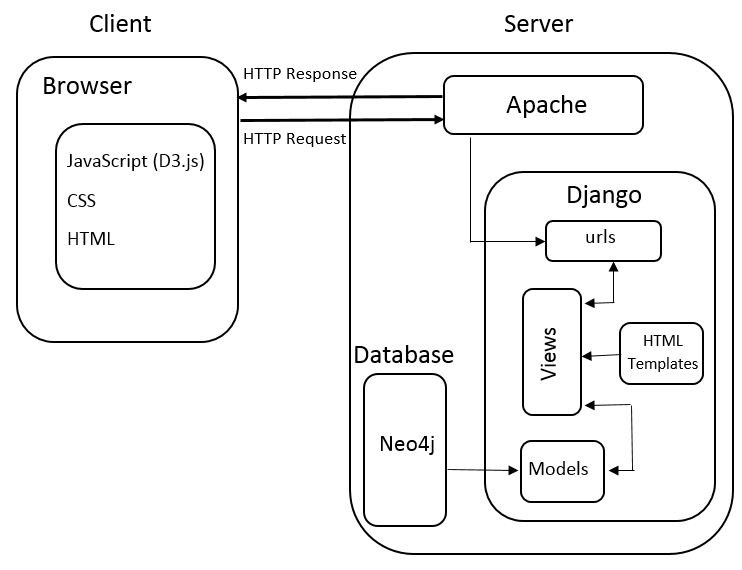
\includegraphics[width=\textwidth]{system}
		\caption{Diagram of System Overview}
		\label{system}
	\end{figure}

	\subsection{Software Development Life Cycle Choice}
	The Software Development Life Cycle (SDLC) is the process or approach the software development team adheres to throughout the project's development. Choosing the correct SDLC for the project is an important decision at the start of a software project as it could determine whether a project is successfully completed within the time frame, budget and scope requirements. A number of common SLDCs were considered:

	\begin{itemize}
		\item \textbf{Waterfall model} - A sequential development model that lacks feedback. This technique consists of the following steps: requirements definition, design, implementation, verification and maintenance. However, due to the lack of feedback, this approach is not feasible unless the requirements are not completely defined in advance, the scope is fixed and the technology is well understood by the development team.

		\item \textbf{Iterative and Incremental process} - A development model in which features are gradually added. Unlike the waterfall approach, this approach makes small changes at a time which can allow for more flexibility. However, this approach still requires the whole system to be well defined at the project start.

		\item \textbf{Agile} - A number of development principles aimed at facilitating the evolution of requirements and solutions in a collaborative process.

	\end{itemize}

	For this particular project, the fast pace method of the Agile SDLC was thought to be the best approach as the pace of producing a working solution is a priority. The requirements for this project have not yet been fully defined and therefore the chosen Agile SDLC must be flexible and able to deal with requirement changes of various sizes.

	The Agile SDLC also has varying methodologies that allows the achievement of an agile software development movement. These methods include the Dynamic System Development Method, the Scrum Method, Rapid Application Development, extreme programming and the Feature-Driven Development Method. The Scrum methodology is the chosen method for this project as it allows the project progression to be agile and flexible with continuous feedback sessions to ensure the requirements are dynamically followed\cite{Kinsey}.

	In the Scrum process, prioritized project tasks (referred to as sprints) are defined in short daily meetings (typically 15 minutes) with all the project team members. These meetings allow the team to communicate project progress and identify the important features that need to be added in order to increase the project progress pace. For this project, these sprints will allow for a working product to be produced in the shortest amount of time while additional features can be  added at a later stage. This process also allows the client to closely keep track of progress and adjust the requirements in order to produce the most high-grade product possible. The daily meeting process occurs for up to 30 days by which time the first release of the developed software should be ready.   


	\subsection{Architecture Choice}
	The choice of software architecture is influenced by the tools and libraries used for both the front-end service and the back-end service (detailed in sections \ref{backsec} and \ref{frontsec}), network communication and team composition. 

	To specify the architecture choice, the team has chosen to follow a two-tier, client-server architecture. In 'client-server', client refers to any user actively interacting with (that is, drawing on for relevant data) the server via the user interface provided by the system. Server refers to the storage and hosting of the integrated software solution on the 'opposite end' of the network, including business and data layer (drawn from the Neo4j graph database). The user interface is only possible with logic on the server. Based on user requests, the logic decides on the correct data to be sent from the server to the client. Having the logic stored on the same server as the database is an important step towards decreasing response time between receiving and fulfilling user request \cite{twotieradvantage}. 

	Two-tier means that any instance of a client utilizing the provided user interface will be separated from the server via a network through which all communication will occur. For the purpose of tracking interconnected Facebook links, the network between the client and the server will be the Internet. This design choice follows the need for multiple users to have access to the software simultaneously \cite{beginningsofteng}. 

	It is important to take note that in this architecture, the client and the server are tightly woven together, as communication between the two entities occurs directly over the network. This means that there is no middle tier to interpret and translate data correctly. In terms of team composition, this design choice is beneficial and reduces the amount of code needed to ensure compatibility. A single, four-man team is working on the software, utilizing an Agile SDLC method that promotes continuous feedback. Due to the small size of the team and the ability to closely work together and ensure quality amongst team work, direct communication between client and server is efficient and easy to achieve.

	\subsection{Front-End Service} \label{frontsec}

	\subsubsection{User Interface Functionality}
	The front-end User Interface (UI) will contain several tools for visualizing Facebook friend networks. The most basic tool will show a simple network diagram to view all friends and friends of friends for the user. This friendship diagram will include several functionalities.

	Firstly, a user may select any of his friends and the diagram will transition to the selected person's friend network. This is pictured in figure \ref{click}. 

	\begin{figure}[htbp]
	    \centering	    
    	\begin{subfigure}[b]{0.3\textwidth}
    		\centering
        	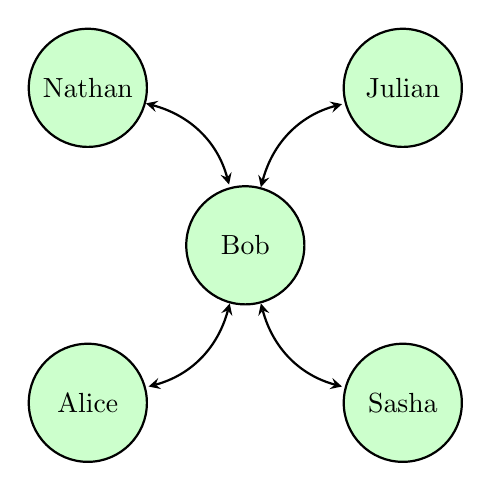
\begin{tikzpicture}[<->,>=stealth,shorten >=1pt,auto,thick,main node/.style={circle,fill=green!20,draw,align=center,minimum width=1.5cm}]

		      \node[main node] at (2,0) (1) {Nathan};
		      \node[main node] at (6,0) (2)  {Julian};
		      \node[main node] at (4,-2) (3) {Bob};
		      \node[main node] at (2,-4) (4) {Alice};
		      \node[main node] at (6,-4) (5) {Sasha};	      

		      \path
		      (1) edge[bend left] (3)
		      (3) edge[bend right] (5)
		      (3) edge[bend left] (4)
		      (3) edge[bend left] (2)   
		      ;

	    	\end{tikzpicture}
        	\caption{Before click}
        	\label{fig:gull1}
    	\end{subfigure}
    	\qquad
    	\qquad
    	\begin{subfigure}[b]{0.3\textwidth}
    		\centering
        	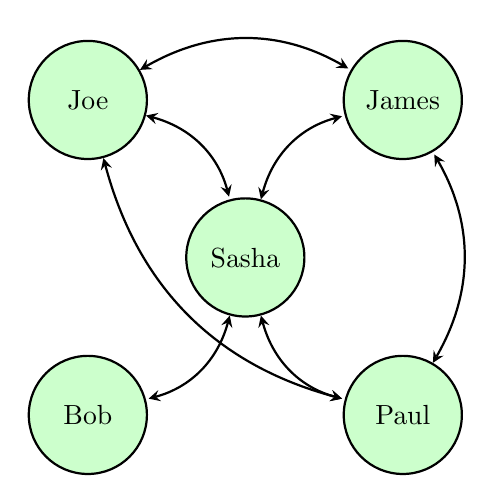
\begin{tikzpicture}[<->,>=stealth,shorten >=1pt,auto,thick,main node/.style={circle,fill=green!20,draw,align=center,minimum width=1.5cm}]
	      
		      \node[main node] at (10,0) (6) {Joe};
		      \node[main node] at (14,0) (7) {James};
		      \node[main node] at (12,-2) (8) {Sasha};
		      \node[main node] at (14,-4) (9) {Paul};
		      \node[main node] at (10,-4) (10) {Bob};      
		    
		      \path
		      (6) edge[bend left] (8)
		      (8) edge[bend right] (9)
		      (8) edge[bend left] (10)
		      (8) edge[bend left] (7)
		      (9) edge[bend right] (7)
		      (6) edge[bend right] (9)
		      (6) edge[bend left] (7)
		      ;

		    \end{tikzpicture}
        	\caption{After click}
        	\label{fig:gull2}
    	\end{subfigure}
	    \caption[Transition of friend network after clicking]{Transition of friend network after clicking on Sasha}
	    \label{click}
	\end{figure}

	Secondly, the user may select certain information to be displayed on the diagram. For example, friendship data can be selected as in figure \ref{details} or relationship data as in figure \ref{relation}.

	\begin{figure}[htbp]
	    \centering
	    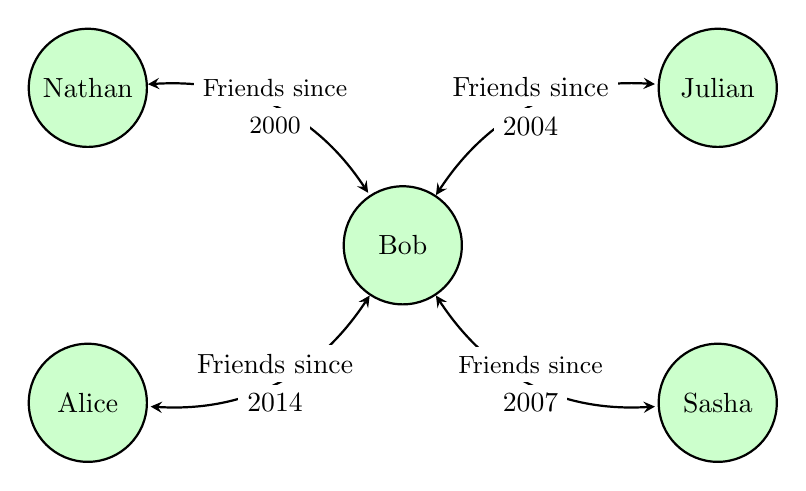
\begin{tikzpicture}[<->,>=stealth,shorten >=1pt,auto,thick,main node/.style={circle,fill=green!20,draw,align=center,minimum width=1.5cm}]

	      \node[main node] at (0,0) (1) {Nathan};
	      \node[main node] at (8,0) (2)  {Julian};
	      \node[main node] at (4,-2) (3) {Bob};
	      \node[main node] at (0,-4) (4) {Alice};
	      \node[main node] at (8,-4) (5) {Sasha};
	          
	      \path
	      (1) edge[bend left] node[above, fill=white] {\small Friends since} node[below,fill=white] {\small 2000} (3)
	      (3) edge[bend right] node[above, fill=white] {\small Friends since} node[below,fill=white] {2007} (5)
	      (3) edge[bend left] node[above,fill=white] {Friends since} node[below,fill=white] {2014} (4)
	      (3) edge[bend left] node[above,fill=white] {Friends since} node[below,fill=white] {2004}(2)
	      ;

	    \end{tikzpicture}
	    \caption{Friend network showing friendship details.}
	    \label{details}
	\end{figure}

	\begin{figure}[htbp]
	    \centering
	    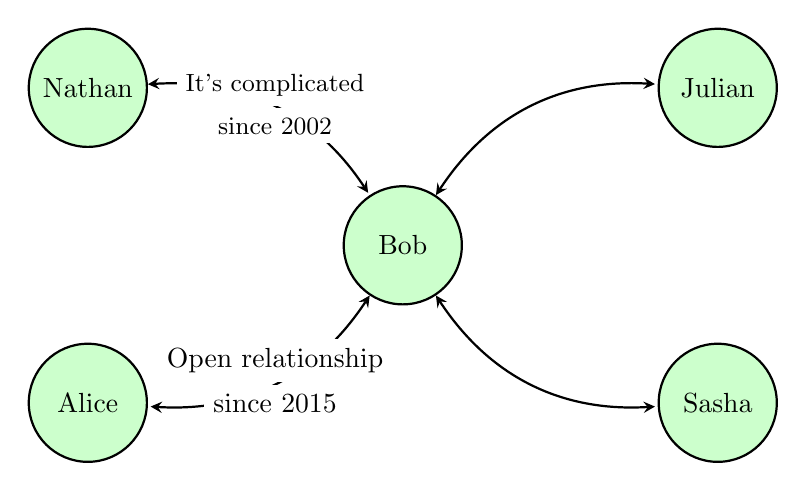
\begin{tikzpicture}[<->,>=stealth,shorten >=1pt,auto,thick,main node/.style={circle,fill=green!20,draw,align=center,minimum width=1.5cm}]

	      \node[main node] at (0,0) (1) {Nathan};
	      \node[main node] at (8,0) (2)  {Julian};
	      \node[main node] at (4,-2) (3) {Bob};
	      \node[main node] at (0,-4) (4) {Alice};
	      \node[main node] at (8,-4) (5) {Sasha};
	          
	      \path
	      (1) edge[bend left] node[above, fill=white] {\small It's complicated} node[below,fill=white] {\small since 2002} (3)
	      (3) edge[bend right] (5)
	      (3) edge[bend left] node[above,fill=white] {Open relationship} node[below,fill=white] {since 2015} (4)
	      (3) edge[bend left] (2)
	      ;

	    \end{tikzpicture}
	    \caption{Friend network showing relationship details.}
	    \label{relation}
	\end{figure}

	Thirdly, the user will be able to show additional information about a user such as their personal information. This is shown in Figure \ref{moreinfo}.

	\begin{figure}[htbp]
	    \centering
	    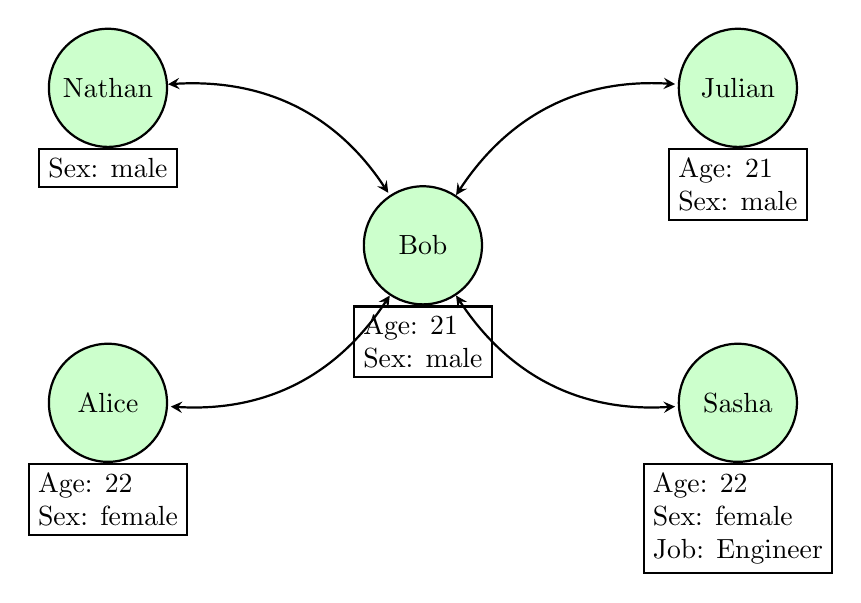
\begin{tikzpicture}[<->,>=stealth,shorten >=1pt,auto,thick,main node/.style={circle,fill=green!20,draw,align=center,minimum width=1.5cm}]

	      \node[main node] at (0,0) (1) {Nathan};
	      \node[main node] at (8,0) (2)  {Julian};
	      \node[main node] at (4,-2) (3) {Bob};
	      \node[main node] at (0,-4) (4) {Alice};
	      \node[main node] at (8,-4) (5) {Sasha};

	      \node[below = 0 cm of 5, fill= white, rectangle, draw, align = left] {Age: 22 \\ Sex: female \\ Job: Engineer};
	      \node[below = 0 cm of 4, fill= white, rectangle, draw, align = left] {Age: 22 \\ Sex: female};
	      \node[below = 0 cm of 3, fill= white, rectangle, draw, align = left] {Age: 21 \\ Sex: male};
	      \node[below = 0 cm of 2, fill= white, rectangle, draw, align = left] {Age: 21 \\ Sex: male};
	      \node[below = 0 cm of 1, fill= white, rectangle, draw, align = left] {Sex: male};
	          
	      \path
	      (1) edge[bend left]  (3)
	      (3) edge[bend right] (5)
	      (3) edge[bend left]  (4)
	      (3) edge[bend left] (2)
	      ;

	    \end{tikzpicture}
	    \caption{Friend network showing personal details.}
	    \label{moreinfo}
	\end{figure}

	Finally, the user will be able customize the types of paths which he would like to show. For example, he or she may want to view only friends in the network who have a certain occupation or gender or age and or any other user attribute. Although it is not shown here the views may be able to display the Facebook profile pictures rather than generic circular nodes.

	\subsubsection{User Interface Implementation}
	The UI will be operated from a web browser. The following sections detail the tools the UI implementation will take advantage of.

	\subsubsection*{HTML and CSS}
	The application will use HTML and CSS to present its content to users. Several HTML pages will be implemented including a landing page, a registration page, a login page, a personal information page, a link to Facebook page and the actual data visualisation pages displaying the friend network and other visualisations.

	\subsubsection*{Bootstrap}
	Bootstrap will be used to style the HTML and CSS pages \cite{Bootstrap}. This will make the UI more user friendly and aesthetically pleasing.

	\subsubsection*{Javascript and d3.js}
	The application will use Javascript and d3.js for visualizing the data \cite{D3}. The friend network diagram will use the D3.js force directed graph. Other d3.js visualisations will also be used for a number of views. Examples of these view include word bubbles for analyses of a user's status messages.

	\subsection{Back-End Service} \label{backsec}

	The back-end will be based on the Django web framework running on an Apache Web Server. The DBMS will be Neo4j, that will be interacted with via the Python driver Py2neo. 
	% \subsubsection{Django}
	% \begin{wrapfigure}{r}{0.2\textwidth}
	%   \begin{center}
	%     
\includegraphics[width=0.25\textwidth]{django}
	%   \end{center}
	%   \caption{The Django Logo}
	% \end{wrapfigure}


	Django is an open source high-level Python Web Framework. It is based on speed, security and scalability. It is also commonly used, with companies such as Mozilla, Pinterest and National Geographic building their websites with it \cite{django}. 

	Although it has its own nomenclature, Django can be considered an MVC (Model View Controller) framework and has been compared to the popular Ruby on Rails web framework. An MVC framework is based on a three layer abstraction. The first layer abstracts the data access of the web application and is called the Model layer. The second layer is responsible for data display and is called the View layer. The final layer regulates the Views and is called the Controller layer. In Django's nomenclature, the view is equivalent to the standard controller, the template is equivalent to the standard view and the model is much the same as usual. For this reason Django is often referred to as a MTV or Model Template View framework \cite{djangobook}. It is important to note that Django is not a programming language, it is a programming pattern designed to streamline web development in the Python programming language.

	Django has its own lightweight web server designed to be used for testing and development. However, for production the Django Software Foundation recommends using Apache with the mod\_wsgi module \cite{djangoApache}.
	\subsubsection{Apache}

	Apache is a free HTTP web server that has been in production since 1995. It is an extremely sophisticated and flexible tool which supports the newest HTTP standards and a large number of platforms \cite{apache}. Apache has a large number of compiled modules that greatly extend it's functionality. 
	% \begin{wrapfigure}{r}{0.2\textwidth}
	%   \begin{center}
	%     
\includegraphics[width=0.25\textwidth]{apache}
	%   \end{center}
	%   \caption{The Apache Logo}
	% \end{wrapfigure}


	Apache processes any incoming HTTP requests from the clients and then sends the appropriate HTTP responses back. This will be done by interfacing with the Django web framework which will make the appropriate decisions based on the requests, and return responses containing content such as information from the Neo4j database. 

	Apache has many functions such as virtual hosting which allow one Apache installation to server multiple websites. This feature allows developers of small websites to save on server costs. Apache also provides many useful security features required when a website goes into production such as: password and digital certificate authentication, SSL and TLS support, and many more. For larger websites Apache also allows load balancing. 

	\subsubsection{Neo4j}
	Neo4j is a graph database written in Java. It is widely used and has drivers for many languages including Python. Neo4j follows the ACID model which means that it is extremely reliable. These statements are evidenced by the use of Neo4j in the systems of large companies such as Walmart and Ebay \cite{neo4j}.  

	Graph databases are a type of NoSQL or Not Only SQL database. They excel at managing large complex sets of data which can be described as nodes and relationships. Figure \ref{neo4eg} shows an example of the type of data that can be stored in a graph database.

	\begin{figure}[htbp]
	    \centering
	    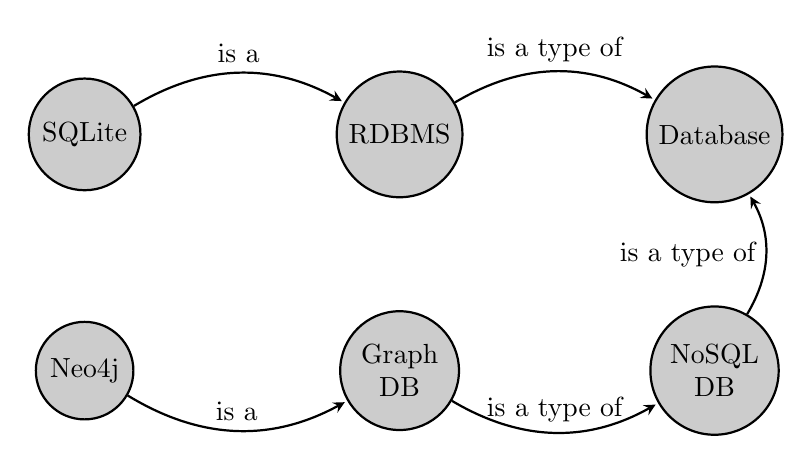
\begin{tikzpicture}[->,>=stealth,shorten >= 1 pt,auto,node distance = 3 cm,
	       thick,main node/.style={circle, fill = black!20 ,draw, align = center}]

	      \node[main node] at (0,0) (1) {Neo4j};
	      \node[main node] at (4,0) (2)  {Graph\\ DB};
	      \node[main node] at (8,0) (3) {NoSQL\\ DB};
	      \node[main node] at (8,3) (4) {Database};
	      \node[main node] at (4,3) (5) {RDBMS};
	      \node[main node] at (0,3) (6) {SQLite};
	      \path
	      (1) edge [bend right] node {is a} (2)
	      (2) edge [bend right] node {is a type of} (3)
	      (3) edge [bend right] node {is a type of} (4)
	      ;
	      \path 
	      (6) edge [bend left] node {is a} (5)
	      (5) edge [bend left] node {is a type of} (4)
	      ;

	    \end{tikzpicture}
	    \caption{Example of data stored in a graph database}
	    \label{neo4eg}
	\end{figure}

	In this application the data being stored will be that of Facebook relationships. Graph databases are orders of magnitudes faster than a RDBMS for queries on this kind of data, such as finding extended friend networks of individuals \cite{graphdbs}.  Figure \ref{friends} shows an example of the kind of data that will be stored in the database.

	\begin{figure}[htbp]
	    \centering
	    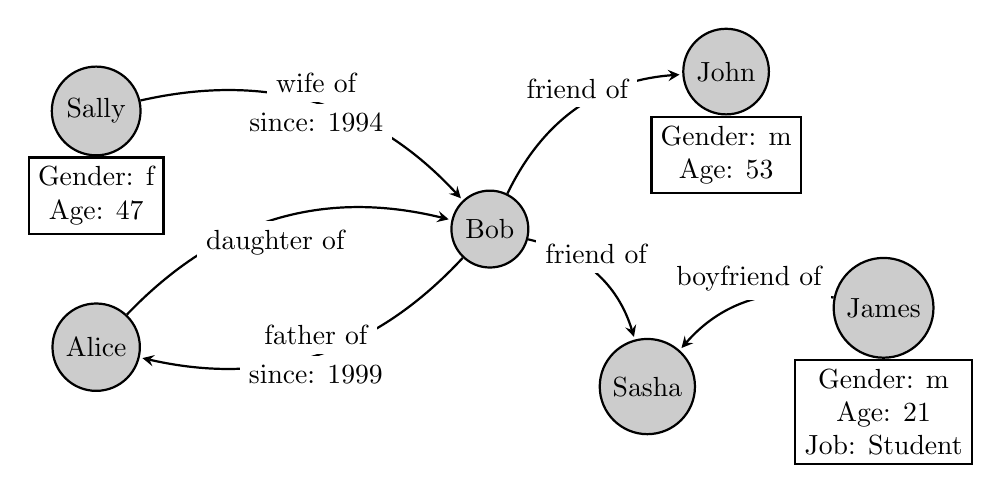
\begin{tikzpicture}[->,>=stealth,shorten >=1pt,auto,thick,main node/.style={circle,fill=black!20,draw,align=center}]

	      \node[main node] at (-1,-0.5) (1) {Sally};
	      \node[draw,rectangle, below = 0cm of 1, align=center,fill=white] (7) {Gender: f\\ Age: 47};
	      \node[main node] at (7,0) (2)  {John};
	      \node[draw,rectangle, below  = 0cm of 2, align=center, fill=white] (6) {Gender: m\\ Age: 53};
	      \node[main node] at (4,-2) (3) {Bob};
	      \node[main node] at (-1,-3.5) (4) {Alice};
	      \node[main node] at (6,-4) (5) {Sasha};
	      \node[main node] at (9,-3) (8) {James};
	      \node[draw,rectangle, below  = 0cm of 8, align=center, fill=white] (9) {Gender: m\\ Age: 21\\ Job: Student};

	    
	      \path
	      (1) edge[bend left] node[above, fill=white] {wife of} node[below,fill=white] {since: 1994} (3)
	      (3) edge[bend left] node[above,fill=white] {friend of} (5)
	      (3) edge[bend left] node[above,fill=white] {father of} node[below,fill=white] {since: 1999} (4)
	      (3) edge[bend left] node[above,fill=white] {friend of} (2)
	      (8) edge[bend right] node[above,fill=white] {boyfriend of} (5)
	      (4) edge[bend left] node[below,fill=white] {daughter of} (3)
	      ;

	    \end{tikzpicture}
	    \caption{Example of facebook type data in a graph database}
	    \label{friends}
	\end{figure}
	Note, from Figure \ref{friends}, that both the relationships as well as the entities themselves have associated data. In fact, each entity acts as a key value store. Queries can be performed to find all friends since a certain date or all friends of friends (as discussed above). These queries can be performed using Neo4j's Cypher query language or via language drivers. The language driver that will be used for this application is Py2neo.

	\subsection{Supporting Software}
	The Interconnected Facebook Links project is intended to be used by a Facebook user and the assumption upon which all user interfaces will be built is that the user is not technologically advanced. Therefore the final product needs to be user friendly and easy to use. The supporting software mentioned in this section describes the technologies that will be used to ensure the aforementioned user-friendliness and functionality of the product is achieved. The framework and internal structure  of the project in terms of the architecture, front-end and back-end has been described in the previous sections. This section describes the software that will be used to support these mentioned structures.

	In order to ensure that the end program is easy to use and looks professional, the visual design and theme needs to have a consistent, well designed layout and be visually appealing. Bootstrap is an HTML, CSS and JavaScript framework that allows this charming front-end visual design to be achieved \cite{Bootstrap}. Bootstrap provides various templates that will maintain the consistent theme throughout the final website. It also provides navigational links for the website and the template is customisable so it can be used to create the desired theme.

	Another technology that will support the functionally of the website is the d3.js JavaScript graphical library \cite{D3}. This library contains JavaScript code for many different visualisation graphs that can be used to visualize the data stored in the Neo4j database. Considering that the main requirement for this project is to visualise the interconnections, the 'force-directed graph' from the d3.js library will be used. As mentioned, other visualisations from the d3.js library can also be used to the further explore the database. These other visualisations include dynamic bar and line charts, geographical heat-maps and dc.js cross-filter graphs, as well as a variety of other options that may be used if they match the functionality appropriately.

	\subsection{Use Cases}
	A number of important use cases describing the base functionality of the product are listed and described in Table \ref{usecase}. These use cases are expanded upon in the Appendix Section \ref{moreusecase}.

	\begin{table} [htbp]
		\caption{Crucial use cases for the product}
		\label{usecase}
		\centering
		\begin{tabular}{p{0.3\textwidth}|p{0.7\textwidth}}
		\hline
		\textbf{Use case} & \textbf{Description} \\ \hline
		log in & The user has to log in in order to access the various views and analytics for their data \\
		sign up & The user has to sign up to be able to log in for the first time \\
		connect to Facebook & The user can connect to their Facebook account to pull data from the Facebook API \\
		upload data & The user can manually upload their friend network data \\
		View friend network & The user views their friend network, showing friends and friends of friends \\
		View friendship data & The user views the details of the friendship links in the friend network view \\
		View relationship data & The user views the details of the relationship links in the friend network view \\
		View personal data & The user views the personal details of their friends in the friend network view \\
		View other visualisations & The user can view other visualisations of their data \\ \hline
		\end{tabular}
	\end{table}

	\begin{figure}[htbp]
		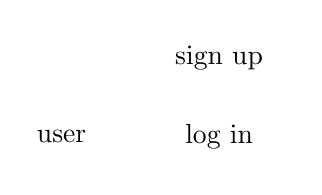
\begin{tikzpicture}[->,>=stealth,draw,fill=white,ultra thick]

			\node at (0,0) (user) {user};
			\node[ellipse] at (2,1) (su) {sign up};
			\node[ellipse] at (2,0) (li) {log in};

		\end{tikzpicture}
		\caption{Use case diagram}
		\label{usecased}
	\end{figure}

\section{The Front-End}	

	\subsection{Design Document} % Joe

	\subsection{Implementation} % Nathan

\section{The Back-End}

	\subsection{Design Document} % Joe

	\subsection{Implementation} % Nathan

\section{Sprint Planning} % Julian

\section{Sprint Retrospective} % Julian

\begin{thebibliography}{1}
	\bibitem{fb} Statista. \url {http://www.statista.com/statistics/264810/number-of-monthly-active-facebook-users-worldwide/}. Last accessed 18 February 2016. 

	\bibitem{pmbok} Project Management Institute. \emph{A Guide to the Project Management Body of Knowledge (PMBOK Guide)}. Newtown Square, Pa: Project Management Institute, 2004. ch 13. p 390.


	\bibitem{Kinsey} H. van Vliet, \emph{Software Engineering: Principles and Practice} Wiley, 2007.
	
	\bibitem{twotieradvantage} N. Liyanage. \emph{Client/Server Architecture: Advantages and Disadvantages of the architectures}. 2013. \url{http://clientserverarch.blogspot.co.za/2013/03/advantages-and-disadvantages-of.html} Last accessed: 9 March 2016
	
	\bibitem{beginningsofteng} R. Stephens, Beginning Software Engineering, 1st ed. Indianapolis: John Wiley And Sons, Inc, 2015, pp. 94-95.
	
	\bibitem{Bootstrap}  \emph{Get Bootstrap - 3.3.6} \url{www.getbootstrap.com} Last accessed: 9 March 2016.
	
	\bibitem{D3}  \emph{d3.js - Data Driven Documents} \url{www.d3.com} Last accessed: 9 March 2016.
	
	\bibitem{django} Django Software Foundation. \emph{Django Overview}. \url{https://www.djangoproject.com/start/overview/}. 2016. Last accessed: 9 March 2016. 
	
	\bibitem{djangobook} Adrian Holovaty, Jacob Kaplan-Moss, et al. \emph{The Django Book}. \url{http://www.djangobook.com/en/2.0/index.html#}. Ch 3. Last accessed: 9 March 2016.
	
	\bibitem{djangoApache} Django Software Foundation. \emph{How to install Django}. \url{https://docs.djangoproject.com/en/1.9/topics/install/}. 2016. Last accessed: 9 March 2016.	
	
	\bibitem{apache} Apache Software Foundation. \emph{Apache - HTTP Server Project}. \url{https://httpd.apache.org/ABOUT_APACHE.html}. 2016. Last accessed: 9 March 2016.	
	
	\bibitem{graphdbs} Robinson I, Webber J, Eifrem E. \emph{Graph Databases} O'Reilly Media. ch 2. pp 21 - 22. June 2013.

	\bibitem{neo4j} neo4j. \url{http://neo4j.com/}, Last accessed 18 February 2016.

	\bibitem{py2neo} Py2Neo. \url{http://py2neo.org/2.0/}, Last accessed 18 February 2016.

	\bibitem{slack} Slack. \url{https://slack.com/}, Last accessed 18 February 2016.

	\bibitem{trello} Trello. \url{https://trello.com/}, Last accessed 18 February 2016.

	\bibitem{wsgi} mod\_wsgi. \url{https://modwsgi.readthedocs.org/en/develop/}, Last accessed 7 April 2016.


\end{thebibliography}

\end{document}